%--------------------------------------
% Spécifications du chat Felix - Camix
%--------------------------------------

\documentclass[a4paper,11pt,titlepage]{article}

\usepackage[english,francais]{babel}
%\usepackage[T1]{fontenc}
\usepackage[utf8]{inputenc}

\usepackage{xspace, graphicx}
\usepackage{amsmath}
\usepackage{amsfonts}
\usepackage{pifont}
\usepackage{lastpage}
\usepackage{listings}
\usepackage{color}

%\usepackage{times}
%\definecolor{grey}{rgb}{0.4,0.4,0.4}

%\usepackage{multicol}
%\usepackage{pifont}

%------------------------------------

\usepackage{fancyhdr}
\usepackage{calc}

\pagestyle{fancy}


\setlength{\hoffset}{-40pt}
\setlength{\topmargin}{-25pt}
\setlength{\headsep}{10pt}

\renewcommand{\headheight}{80pt}

\renewcommand{\headwidth}{450pt}
\setlength{\textwidth}{450pt}
\setlength{\textheight}{604pt}

\renewcommand{\footrulewidth}{0.1mm}

\fancyhf{}
        %\fancyhead[LO]{\bf \includegraphics[width=60pt]{../img/logoeseo.eps} \includegraphics[width=130pt]{../img/logoemn.eps}}
        \fancyhead[LO]{\bf 
\includegraphics[width=60pt]{../img/logo_eseo.eps}}
	\fancyhead[RO]{\bf {\large Logiciel \og Chat \fg\\
				{\large Spécifications}\\
				{\small\textit{version du \today}}}}
        \fancyfoot[LO]{\sl Chat \og Felix - Camix \fg}
	\fancyfoot[RO]{\thepage/\pageref{LastPage}}

%---------------------------------------
\lstset{
	basicstyle=\footnotesize\ttfamily,
	commentstyle=\small\itshape\color[gray]{0.5},
	morecomment=[l]Remarque,
	showlines=false,
	frame=lines,
	xleftmargin=4mm,
	framexleftmargin=4mm,
	xrightmargin=4mm,
	framexrightmargin=4mm,
	framextopmargin=1mm,
	framexbottommargin=1mm,
	backgroundcolor=\color[gray]{0.98},
	rulesep=6pt,
	captionpos=b,
	abovecaptionskip=\medskipamount,
	belowcaptionskip=\bigskipamount,
	numbers=none,
	tabsize=4,
	literate=
		{á}{{\'a}}1 {é}{{\'e}}1 {í}{{\'i}}1 {ó}{{\'o}}1 {ú}{{\'u}}1
		{Á}{{\'A}}1 {É}{{\'E}}1 {Í}{{\'I}}1 {Ó}{{\'O}}1 {Ú}{{\'U}}1
		{à}{{\`a}}1 {è}{{\`e}}1 {ì}{{\`i}}1 {ò}{{\`o}}1 {ù}{{\`u}}1
		{À}{{\`A}}1 {È}{{\'E}}1 {Ì}{{\`I}}1 {Ò}{{\`O}}1 {Ù}{{\`U}}1
		{ä}{{\"a}}1 {ë}{{\"e}}1 {ï}{{\"i}}1 {ö}{{\"o}}1 {ü}{{\"u}}1
		{Ä}{{\"A}}1 {Ë}{{\"E}}1 {Ï}{{\"I}}1 {Ö}{{\"O}}1 {Ü}{{\"U}}1
		{â}{{\^a}}1 {ê}{{\^e}}1 {î}{{\^i}}1 {ô}{{\^o}}1 {û}{{\^u}}1
		{Â}{{\^A}}1 {Ê}{{\^E}}1 {Î}{{\^I}}1 {Ô}{{\^O}}1 {Û}{{\^U}}1
		{ã}{{\~a}}1 {Ã}{{\~A}}1 {õ}{{\~o}}1 {Õ}{{\~O}}1
		{œ}{{\oe}}1 {Œ}{{\OE}}1 {æ}{{\ae}}1 {Æ}{{\AE}}1 {ß}{{\ss}}1
		{ç}{{\c c}}1 {Ç}{{\c C}}1 {ø}{{\o}}1 {å}{{\r a}}1 {Å}{{\r A}}1
		{€}{{\EUR}}1 {£}{{\pounds}}1
}

%---------------------------------------
\setcounter{tocdepth}{3}

%----------------------------------------
%	DOCUMENT
%----------------------------------------

\begin{document}

%------- MISE EN PAGE STRICT -----------
\sloppy%

%---------------------------------------
\vspace{-2cm}%
\begin{center}%

\vspace{0.2cm}
{\Large {\textsc{\bf Logiciel \og Chat \fg}}}

\rule[0.5ex]{0.52\textwidth}{0.1mm}

\vspace{0.2cm}
{\Large\bf{Spécifications}}

\rule[0.5ex]{0.52\textwidth}{0.1mm}
\end{center}

\vspace{1cm}
\begin{tabular}{|p{5cm}|p{9cm}|}
\hline
\textbf{Auteur} & \textbf{Contact} \\
\hline
Matthias Brun & matthias.brun@eseo.fr\\
\hline
\end{tabular}

\vspace{0.5cm}
\begin{tabular}{|p{5cm}|p{9cm}|}
\hline
\textbf{Relecteur} & \textbf{Contact} \\
\hline
Camille Constant & camille.constant@eseo.fr\\
\hline
\end{tabular}

\vspace{0.5cm}
\begin{tabular}{|p{5cm}|p{9cm}|}
	\hline
	\textbf{Testeurs} & \textbf{Contact} \\
	\hline
	Younes Ghoniem & younes.ghoniem@imt-atlantique.net\\
	\hline
	Matthieu Schmitz & matthieu.schmitz@imt-atlantique.net\\
	\hline
\end{tabular}

\vspace{1cm}
\begin{tabular}{|p{1.5cm}|p{2cm}|p{10.1cm}|}
\hline
\textbf{Version} & \textbf{Date} & \textbf{Commentaire} \\
\hline
1.0 & 14/04/2023 & Ajout Specifications; \newline
			Ajout TU ; \newline
			Ajout Tests Utilisateurs. \\
0.6 & 14/02/2022 & Modifications Déploiement ; \newline
			Modifications IHM messages textuels.\\
0.5 & 22/01/2018 & Modifications Domaine ; \newline
			Modifications IHM messages du serveur $\rightarrow$ messages textuels.\\
0.4 & 19/02/2017 & Ajout Domaine ; \newline
			Modifications Introduction ; \newline
			Modifications CU ; \newline
			Modifications IHM. \\
0.3 & 13/01/2013 & Ajout CU sortir du chat ; \newline
			Modification CU lancement client chat $\rightarrow$ entrer dans le chat ; \newline
			Modifications IHM : Messages du serveur.\\
0.2 & 09/01/2013 & Ajout CU lancement client chat ; \newline
			Ajout pré-conditions aux CU ; \newline 
			Modifications IHM : Messages du serveur.\\
0.1 & 08/01/2013 & Introduction, Déploiement, CU, IHM.\\
\hline
\end{tabular}
\newpage

%------------------------------- 

\tableofcontents
% alternative pour réduire l'espacement entre les entrées de la table des matières 
% (la valeur numérique peut être adaptée au besoin) : 
%{\setlength{\baselineskip}{0.9\baselineskip}\tableofcontents\par}
\newpage

%-------------------------------

%--------------------------------------
% Spécifications du chat Felix - Camix
%
% Introduction
%--------------------------------------

\section{Introduction}
\label{sec:introduction}

\subsection{Objectif des spécifications}
\label{subsec:introduction:objectif}

Ce document spécifie un ensemble logiciel composé d'un serveur et de clients chat.
Plusieurs clients chat peuvent se connecter au serveur chat et échanger des messages textuels via ce serveur.

\smallskip
Ce document décrit en particulier :
\begin{itemize}
\smallskip
\item \textbf{le déploiement} prévu des composants serveur et clients chat ;
\smallskip
\item \textbf{le domaine} d'application du chat ;
\smallskip
\item \textbf{les cas d'utilisation} attendus pour cet ensemble logiciel ;
\smallskip
\item \textbf{l'interface homme-machine} envisagée pour un client ainsi que le protocole de communication client/serveur et les messages renvoyés par le serveur.
\smallskip
\item \textbf{Les spécifications clients} revues et validées par les clients puis appliquées et testées.
\end{itemize}


\subsection{Portée des spécifications}
\label{subsec:introduction:portee}

Ce document concerne tous les intervenants du projet.

\subsection{Modification des spécifications}
\label{subsec:introdtion:modification}

Les spécifications pourront être soumises à des modifications. 
Toute nouvelle version sera signalée par mail à l'ensemble des intervenants du projet.


\newpage

%--------------------------------------
% Spécifications du chat Felix - Camix
%
% Déploiement
%--------------------------------------

\section{Déploiement}
\label{sec:deploiement}

Le chat se compose de deux entités : les composants logiciels \textbf{Camix} et \textbf{Felix} (cf. figure~\ref{sec:deploiement:figchat}), respectivement composant serveur et client du chat.

\smallskip
Les composants Camix et Felix sont programmés en Java. Leurs exécutions nécessitent une machine virtuelle Java (ou \textit{Java Virtual Machine} - JVM) en version supérieure ou égale 8.

\smallskip
Les composants Felix et Camix communiquent via un réseau TCP/IP (\textit{Transmission Control Protocol/Internet Protocol}).

\medskip
\begin{figure}[h!]
\begin{center}
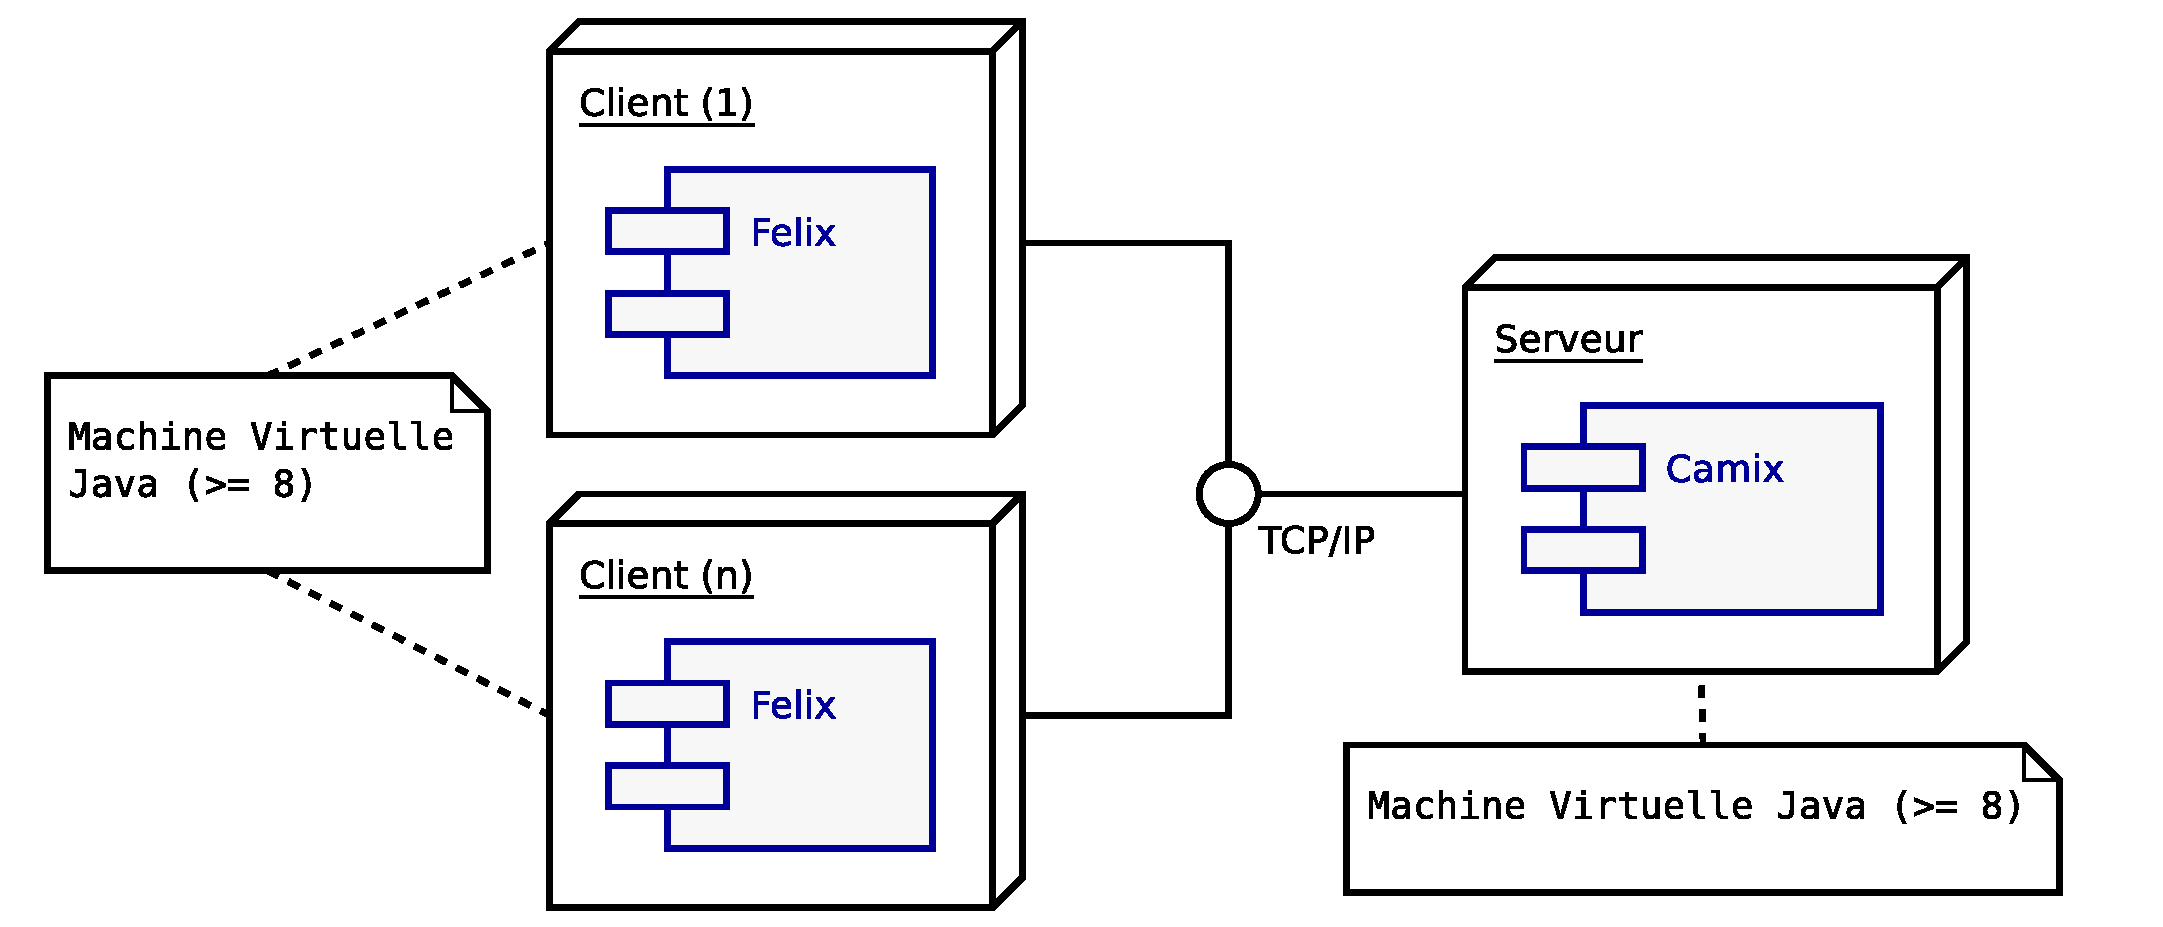
\includegraphics[width=\linewidth]{../img/Chat_Deploiement.eps}
\caption{Diagramme de déploiement du chat.}
\label{sec:deploiement:figchat}
\end{center}
\end{figure}



\vspace{-0.5cm}
%--------------------------------------
% Spécifications du chat Felix - Camix
%
% Domaine
%--------------------------------------

\section{Domaine}
\label{sec:domaine}

Un chat est muni de canaux pouvant accueillir des utilisateurs (cf. figure~\ref{sec:domaine:figchat}). Les utilisateurs peuvent communiquer entre eux au sein d'un même canal. Un utilisateur est reconnu par les autres utilisateurs par son surnom. Le surnom par défaut est un point d'interrogation (\texttt{?}). Un canal est identifié par son nom.

\medskip
\begin{figure}[h!]
\begin{center}
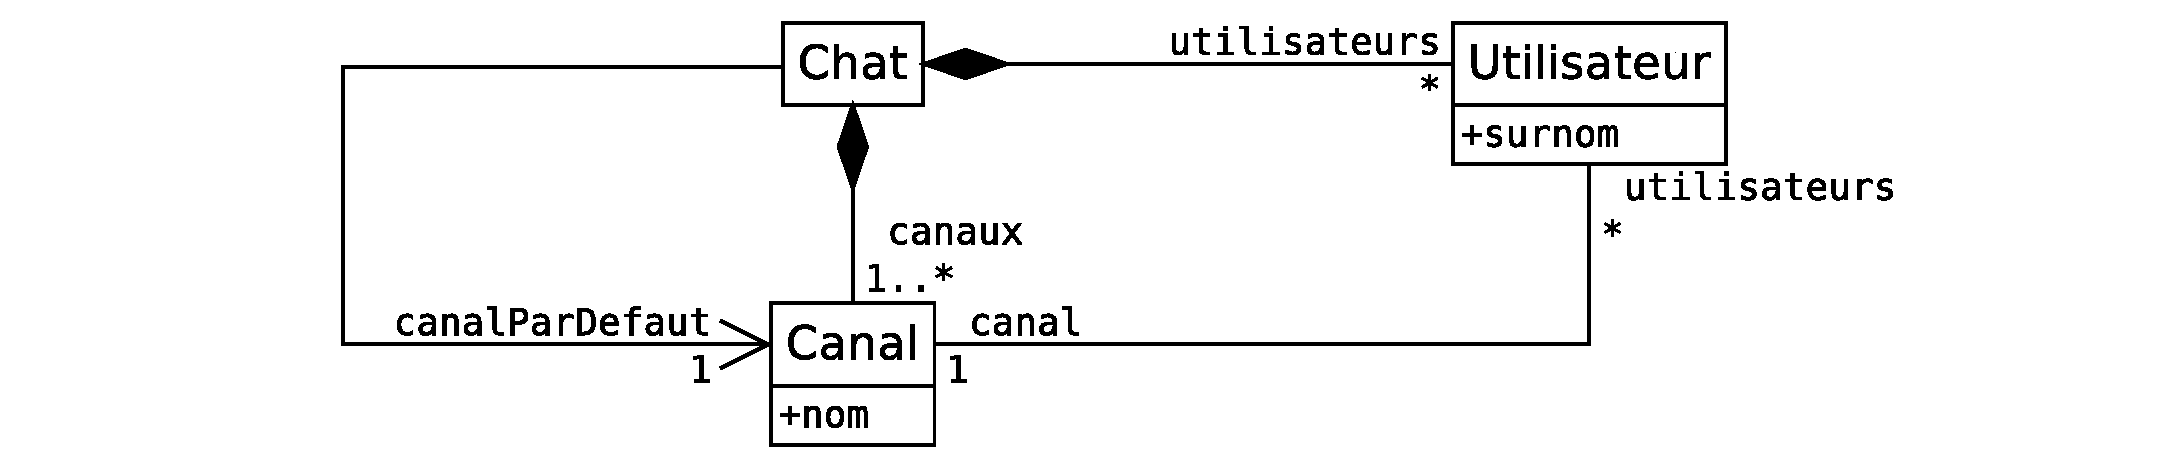
\includegraphics[width=\linewidth]{../img/Chat_Domaine.eps}
\caption{Diagramme de classes du domaine du chat.}
\label{sec:domaine:figchat}
\end{center}
\end{figure}


\newpage

%--------------------------------------
% Spécifications du chat Felix - Camix
%
% CU
%--------------------------------------

\section{Cas d'utilisation}
\label{sec:cu}

La figure~\ref{sec:cu:figcu} présente les cas d'utilisation du chat.

\medskip
\begin{figure}[h!]
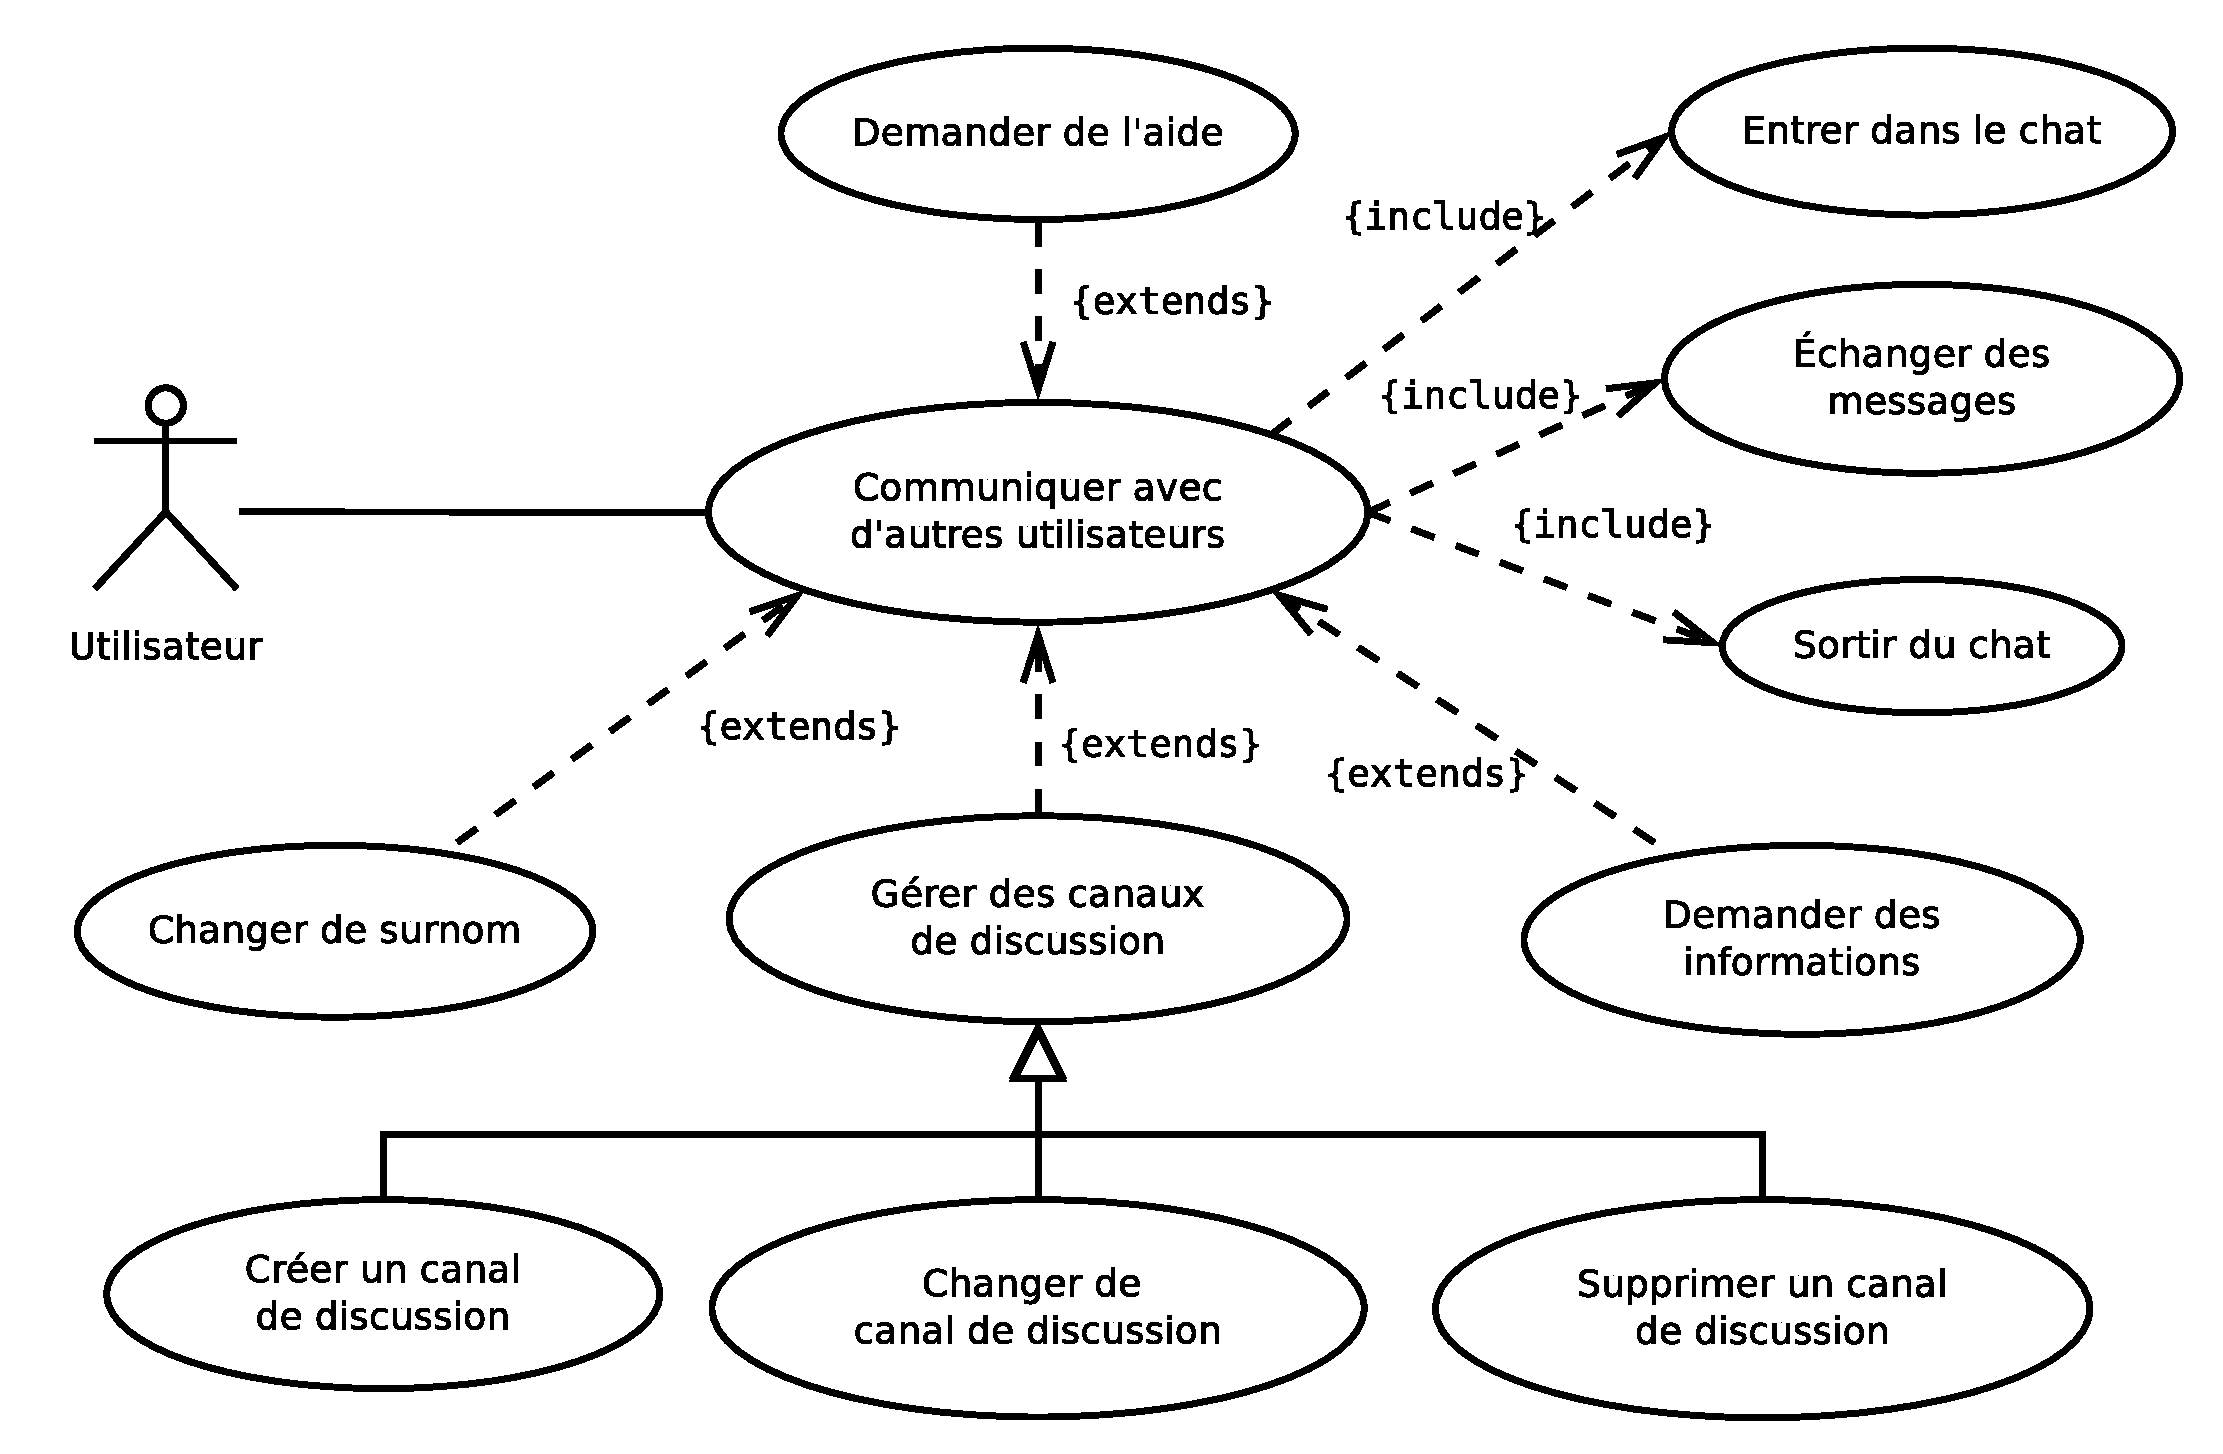
\includegraphics[width=\linewidth]{../img/Chat_CU.eps}
\caption{Cas d'utilisation du chat.}
\label{sec:cu:figcu}
\end{figure}

\medskip
Chacun de ces cas d'utilisation est détaillé dans la suite de cette section.

\subsection{Communiquer avec d'autres utilisateurs}
\label{sec:cu:communiquer}

L'objectif du chat est de permettre à des utilisateurs de communiquer entre eux. Après être entré dans le chat, cette communication se fait par échanges de messages textuels. Chaque utilisateur est identifié par les autres utilisateurs via un surnom qu'il peut changer au cours de son utilisation du chat. Les échanges de messages se font au sein de canaux de discussion dont une gestion est possible par chaque utilisateur (création, suppression et changement de canal). Enfin, le chat fournit une aide aux utilisateurs ainsi que des informations sur les canaux existants et sur les utilisateurs eux-mêmes. La sortie du chat se fait en fermant le client chat (Felix).

\medskip
Remarque (1) : Un serveur chat (Camix) compatible avec le client chat (Felix) doit être lancé pour permettre aux différents utilisateurs de communiquer.

\smallskip
Remarque (2) : Pour utiliser les différentes fonctionnalités du chat, un protocole est à la disposition des utilisateurs. Ce protocole (spécifié dans la section~\ref{sec:ihm:protocole}, page~\pageref{sec:ihm:protocole}) définit un ensemble de commandes que peut invoquer un utilisateur.

\medskip
\noindent
Cas d'utilisation : Communiquer avec d'autres utilisateurs.\\
Résumé : Un utilisateur lance un client chat pour entrer dans le chat, il peut ensuite échanger des messages, demander de l'aide sur les commandes du chat, changer de surnom, demander des informations, gérer des canaux de discussion et sortir du chat. \\
Niveau : Stratégique.\\
Acteur principal : Utilisateur.\\
Acteurs secondaires : Les autres utilisateurs du chat.\\
Pré-conditions : Un logiciel serveur (Camix) est lancé et accessible par le réseau TCP/IP.

\medskip
\textbf{Scénario nominal} :
\begin{enumerate}
\item L'utilisateur \underline{entre dans le chat} (cf. \ref{sec:cu:entrerchat}, page~\pageref{sec:cu:entrerchat}).
\item L'utilisateur \underline{échange des messages} avec les autres utilisateurs du chat (cf. \ref{sec:cu:echange}, page~\pageref{sec:cu:echange}).
\item L'utilisateur \underline{sort du chat} (cf. \ref{sec:cu:sortirchat}, page~\pageref{sec:cu:sortirchat}).
\end{enumerate}

\medskip
\textbf{Variantes} :
\begin{enumerate}
\item[2.a] L'utilisateur \underline{demande de l'aide} (cf. \ref{sec:cu:aide}, page~\pageref{sec:cu:aide}).
\item[2.b] L'utilisateur \underline{change de surnom} (cf. \ref{sec:cu:changersurnom}, page~\pageref{sec:cu:changersurnom}).
\item[2.c] L'utilisateur \underline{demande des informations} (cf. \ref{sec:cu:informations}, page~\pageref{sec:cu:informations}).
\item[2.d] L'utilisateur \underline{gère des canaux de discussion} (cf. \ref{sec:cu:canaux}, page~\pageref{sec:cu:canaux}).
\end{enumerate}

\medskip
\textbf{Exception} [Commande invalide] :
\begin{enumerate}
\item[2.e] L'utilisateur \underline{saisit une commande invalide} (cf. \ref{sec:cu:cmdinvalide}, page~\pageref{sec:cu:cmdinvalide}).
\end{enumerate}


\subsection{Entrer dans le chat}
\label{sec:cu:entrerchat}

\noindent
Cas d'utilisation : Entrer dans le chat.\\
Résumé : Un utilisateur entre dans le chat en lançant le logiciel client du chat.\\
Acteur principal : Utilisateur.\\
Acteurs secondaires : Les autres utilisateurs du chat.\\
Pré-conditions : Un logiciel serveur (Camix) est lancé et accessible par le réseau TCP/IP.

\medskip
\textbf{Scénario nominal} :
\begin{enumerate}
\item L'utilisateur lance l'exécution du composant Felix.
\item Felix initie la connexion à Camix.
\item Camix inscrit l'utilisateur dans le canal par défaut (place publique).
\item Camix informe les composants Felix des autres utilisateurs inscrits dans le canal par défaut que l'utilisateur arrive dans le chat.
\item Chaque composant Felix concerné affiche un message d'arrivée de l'utilisateur dans le chat.
\item Camix transmet au composant Felix de l'utilisateur un message d'accueil dans le chat.
\item Felix affiche un message d'accueil dans le chat.
\end{enumerate}
 
\subsection{Demander de l'aide}
\label{sec:cu:aide}

\noindent
Cas d'utilisation : Demander de l'aide.\\
Résumé : Un utilisateur peut demander de l'aide sur les commandes du chat. \\
Acteur principal : Utilisateur.\\
Pré-conditions : Le composant client du chat (Felix) est lancé et connecté par TCP/IP au composant serveur du chat (Camix).

\textbf{Scénario nominal} :
\begin{enumerate}
\item L'utilisateur saisit la commande d'aide.
\item Felix transmet la commande d'aide à Camix.
\item Camix transmet à Felix les informations sur les commandes disponibles.
\item Felix affiche un message d'aide sur les commandes disponibles.
\end{enumerate}

\subsection{Échanger des messages}
\label{sec:cu:echange}

\noindent
Cas d'utilisation : Échanger des messages.\\
Résumé : Un utilisateur échange des messages avec d'autres utilisateurs. \\
Acteur principal : Utilisateur.\\
Acteurs secondaires : Les autres utilisateurs du chat.\\
Pré-conditions : Le composant client du chat (Felix) est lancé et connecté par TCP/IP au composant serveur du chat (Camix).

\medskip
\textbf{Scénario nominal} :
\begin{enumerate}
\item L'utilisateur saisit un message textuel.
\item Felix transmet le message à Camix.
\item Camix transmet le message aux composants Felix des utilisateurs inscrits dans le même canal que celui de l'utilisateur.
\item Chaque composant Felix concerné affiche le message.
\end{enumerate}

\subsection{Changer de surnom}
\label{sec:cu:changersurnom}

Les utilisateurs peuvent avoir des surnoms pour être plus facilement identifiés dans le chat. Le surnom par défaut d'un utilisateur est un point d'interrogation (\texttt{?}).

\medskip
\noindent
Cas d'utilisation : Changer de surnom.\\
Résumé : Un utilisateur change de surnom.\\
Acteur principal : Utilisateur.\\
Acteurs secondaires : Les autres utilisateurs du chat.\\
Pré-conditions : Le composant client du chat (Felix) est lancé et connecté par TCP/IP au composant serveur du chat (Camix).

\medskip
\textbf{Scénario nominal} :
\begin{enumerate}
\item L'utilisateur saisit la commande de changement de surnom.
\item Felix transmet la commande de changement de surnom à Camix.
\item Camix change le surnom de l'utilisateur.
\item Camix informe les composants Felix des utilisateurs inscrits dans le même canal que celui de l'utilisateur que ce dernier a changé de surnom.
\item Chaque composant Felix concerné affiche un message de changement de surnom de l'utilisateur.
\end{enumerate}

\subsection{Demander des informations}
\label{sec:cu:informations}

Le serveur chat peut fournir à chaque utilisateur des informations personnelles (surnom de l'utilisateur et canal occupé) et sur les canaux du chat (noms et nombres d'utilisateurs).  

\medskip
\noindent
Cas d'utilisation : Demander des informations.\\
Résumé : Un utilisateur peut faire afficher ses informations personnelles ou des informations sur les canaux du chat. \\
Acteur principal : Utilisateur.\\
Pré-conditions : Le composant client du chat (Felix) est lancé et connecté par TCP/IP au composant serveur du chat (Camix).

\medskip
\textbf{Scénario nominal} :
\begin{enumerate}
\item L'utilisateur \underline{demande ses informations personnelles} (cf. \ref{sec:cu:informations:personnelles}, page~\pageref{sec:cu:informations:personnelles}).
\end{enumerate}

\medskip
\textbf{Variante} :
\begin{enumerate}
\item[1.a] L'utilisateur \underline{demande les informations sur les canaux} (cf. \ref{sec:cu:informations:canaux}, page~\pageref{sec:cu:informations:canaux}).
\end{enumerate}

\subsubsection{Demander ses informations personnelles}
\label{sec:cu:informations:personnelles}

\noindent
Cas d'utilisation : Demander des informations personnelles.\\
Résumé : Un utilisateur peut obtenir ses informations personnelles (surnom et canal occupé). \\
Acteur principal : Utilisateur.\\
Pré-conditions : Le composant client du chat (Felix) est lancé et connecté par TCP/IP au composant serveur du chat (Camix).

\medskip
\textbf{Scénario nominal} :
\begin{enumerate}
\item L'utilisateur saisit la commande d'informations personnelles.
\item Felix transmet la commande d'informations personnelles à Camix.
\item Camix transmet à Felix les informations sur l'utilisateur (surnom et canal occupé).
\item Felix affiche les informations personnelles de l'utilisateur.
\end{enumerate}

\subsubsection{Demander les informations sur les canaux}
\label{sec:cu:informations:canaux}

\noindent
Cas d'utilisation : Demander des informations sur les canaux.\\
Résumé : Un utilisateur peut obtenir des informations sur les canaux de discussion (noms et nombres d'utilisateurs). \\
Acteur principal : Utilisateur.\\
Pré-conditions : Le composant client du chat (Felix) est lancé et connecté par TCP/IP au composant serveur du chat (Camix).

\medskip
\textbf{Scénario nominal} :
\begin{enumerate}
\item L'utilisateur saisit la commande d'informations sur les canaux.
\item Felix transmet la commande d'informations sur les canaux à Camix.
\item Camix transmet à Felix les informations sur les canaux (noms et nombres d'utilisateurs).
\item Felix affiche les informations sur les canaux.
\end{enumerate}

\subsection{Gérer des canaux de discussion}
\label{sec:cu:canaux}

Le serveur chat offre la possibilité d'échanger des messages dans des canaux de discussion. 
Les échanges au sein d'un canal restent internes à celui-ci, ils ne sont pas visibles des autres canaux. Le canal par défaut du serveur chat se nomme \texttt{place publique}. Le serveur permet de créer et de supprimer des canaux de discussion ainsi que de changer de canal de discussion lors de l'utilisation du chat.

\medskip
\noindent
Cas d'utilisation : Gérer des canaux de discussion.\\
Résumé : Un utilisateur peut créer des canaux de discussion, changer de canal de discussion et supprimer des canaux de discussion. \\
Acteur principal : Utilisateur.\\
Pré-conditions : Le composant client du chat (Felix) est lancé et connecté par TCP/IP au composant serveur du chat (Camix).

\medskip
\textbf{Scénario nominal} :
\begin{enumerate}
\item L'utilisateur \underline{crée un canal de discussion} (cf. \ref{sec:cu:canaux:creer}, page~\pageref{sec:cu:canaux:creer}).
\end{enumerate}

\medskip
\textbf{Variantes} :
\begin{enumerate}
\item[1.a] L'utilisateur \underline{supprime un canal de discussion} (cf. \ref{sec:cu:canaux:supprimer}, page~\pageref{sec:cu:canaux:supprimer}).
\item[1.b] L'utilisateur \underline{change de canal de discussion} (cf. \ref{sec:cu:canaux:changer}, page~\pageref{sec:cu:canaux:changer}).
\end{enumerate}


\subsubsection{Créer un canal de discussion}
\label{sec:cu:canaux:creer}

\noindent 
Cas d'utilisation : Créer un canal de discussion.\\
Résumé : Un utilisateur crée un canal de discussion sur le serveur du chat.\\
Acteur principal : Utilisateur.\\
Pré-conditions : Le composant client du chat (Felix) est lancé et connecté par TCP/IP au composant serveur du chat (Camix).

\medskip
\textbf{Scénario nominal} :
\begin{enumerate}
\item L'utilisateur saisit la commande de création d'un canal.
\item Felix transmet la commande de création du canal à Camix.
\item Camix crée le canal.
\item Camix informe Felix qu'un canal a été créé.
\item Felix affiche un message de création du canal.
\end{enumerate}

\newpage
\textbf{Exception} [le canal existe déjà] :
\begin{enumerate}
\item[3.a.1] Camix informe Felix que le canal existe déjà.
\item[3.a.2] Felix affiche un message d'existence du canal.
\item[3.a.3] Fin du CU.
\end{enumerate}

\subsubsection{Supprimer un canal de discussion}
\label{sec:cu:canaux:supprimer}

\noindent
Cas d'utilisation : Supprimer un canal de discussion.\\
Résumé : Un utilisateur supprime un canal de discussion sur le serveur du chat.\\
Acteur principal : Utilisateur.\\
Pré-conditions : Le composant client du chat (Felix) est lancé et connecté par TCP/IP au composant serveur du chat (Camix). Un canal de discussion autre que le canal par défaut a été créé dans le chat.

\medskip
\textbf{Scénario nominal} :
\begin{enumerate}
\item L'utilisateur saisit la commande de suppression d'un canal.
\item Felix transmet la commande de suppression du canal à Camix.
\item Camix supprime le canal.
\item Camix informe Felix qu'un canal a été supprimé.
\item Felix affiche un message de suppression du canal.
\end{enumerate}

\medskip
\textbf{Exception} [le canal n'existe pas] :
\begin{enumerate}
\item[3.a.1] Camix informe Felix que le canal n'existe pas.
\item[3.a.2] Felix affiche un message de non existence du canal.
\item[3.a.3] Fin du CU.
\end{enumerate}

\medskip
\textbf{Exception} [le canal n'est pas vide] :
\begin{enumerate}
\item[3.b.1] Camix informe Felix que le canal n'est pas vide.
\item[3.b.2] Felix affiche un message de canal non vide.
\item[3.b.3] Fin du CU.
\end{enumerate}

\medskip
\textbf{Exception} [le canal est le canal par défaut (\texttt{place publique})] :
\begin{enumerate}
\item[3.c.1] Camix informe Felix que le canal ne peut pas être supprimé.
\item[3.c.2] Felix affiche un message de canal non supprimable.
\item[3.c.3] Fin du CU.
\end{enumerate}

\subsubsection{Changer de canal de discussion}
\label{sec:cu:canaux:changer}

\noindent
Cas d'utilisation : Changer de canal de discussion.\\
Résumé : Un utilisateur change de canal de discussion sur le serveur du chat.\\
Acteur principal : Utilisateur.\\
Acteurs secondaires : Les autres utilisateurs du chat.\\
Pré-conditions : Le composant client du chat (Felix) est lancé et connecté par TCP/IP au composant serveur du chat (Camix). Un canal de discussion autre que le canal par défaut a été créé dans le chat.

\newpage
\textbf{Scénario nominal} :
\begin{enumerate}
\item L'utilisateur saisit la commande de changement de canal.
\item Felix transmet la commande de changement de canal à Camix.
\item Camix informe les composants Felix des utilisateurs inscrits dans le même canal que celui de l'utilisateur que ce dernier quitte le canal.
\item Chaque composant Felix concerné affiche un message de départ de l'utilisateur du canal.
\item Camix change l'utilisateur de canal.
\item Camix informe les composants Felix des utilisateurs inscrits dans le nouveau canal de l'utilisateur que celui-ci arrive dans le canal.
\item Chaque composant Felix concerné affiche un message d'arrivée de l'utilisateur dans le canal.
\end{enumerate}

\textbf{Exception} [le canal n'existe pas] :
\begin{enumerate}
\item[3.a.1] Camix informe Felix que le canal n'existe pas.
\item[3.a.2] Felix affiche un message de non existence du canal demandé.
\item[3.a.3] Fin du CU.
\end{enumerate}


\subsection{Sortir du chat}
\label{sec:cu:sortirchat}

\noindent
Cas d'utilisation : Sortir du chat.\\
Résumé : Un utilisateur sort du chat en fermant le logiciel client du chat.\\
Acteur principal : Utilisateur.\\
Acteurs secondaires : Les autres utilisateurs du chat.\\
Pré-conditions : Le composant client du chat (Felix) est lancé et connecté par TCP/IP au composant serveur du chat (Camix).

\medskip
\textbf{Scénario nominal} :
\begin{enumerate}
\item L'utilisateur arrête l'exécution du composant Felix.
\item Felix se déconnecte de Camix.
\item Camix informe les composants Felix des utilisateurs inscrits dans le même canal que celui de l'utilisateur que ce dernier quitte le chat.
\item Chaque composant Felix concerné affiche un message de départ de l'utilisateur du chat.
\item Camix désinscrit l'utilisateur du canal dans lequel il se trouve.
\item Camix ferme la connexion de l'utilisateur.
\end{enumerate}

\subsection{Saisir une commande invalide}
\label{sec:cu:cmdinvalide}

\noindent
Cas d'utilisation : Saisir une commande invalide.\\
Résumé : Un utilisateur peut obtenir de l'aide sur les commandes du chat s'il saisit une commande invalide. \\
Acteur principal : Utilisateur.\\
Pré-conditions : Le composant client du chat (Felix) est lancé et connecté par TCP/IP au composant serveur du chat (Camix).

\newpage
\textbf{Scénario nominal} :
\begin{enumerate}
\item L'utilisateur saisit une commande invalide.
\item Felix transmet la commande à Camix.
\item Camix transmet à Felix les informations sur les commandes disponibles.
\item Felix affiche un message d'aide sur les commandes disponibles.
\end{enumerate}


\newpage

%--------------------------------------
% Spécifications du chat Felix - Camix
%
% IHM
%--------------------------------------

\section{Interface homme-machine}
\label{sec:ihm}

\subsection{Interface homme-machine de Felix}
\label{sec:ihm:felix}

La figure~\ref{sec:ihm:felix:fig} présente l'interface homme-machine (IHM) du client chat Felix.

\begin{figure}[h!]
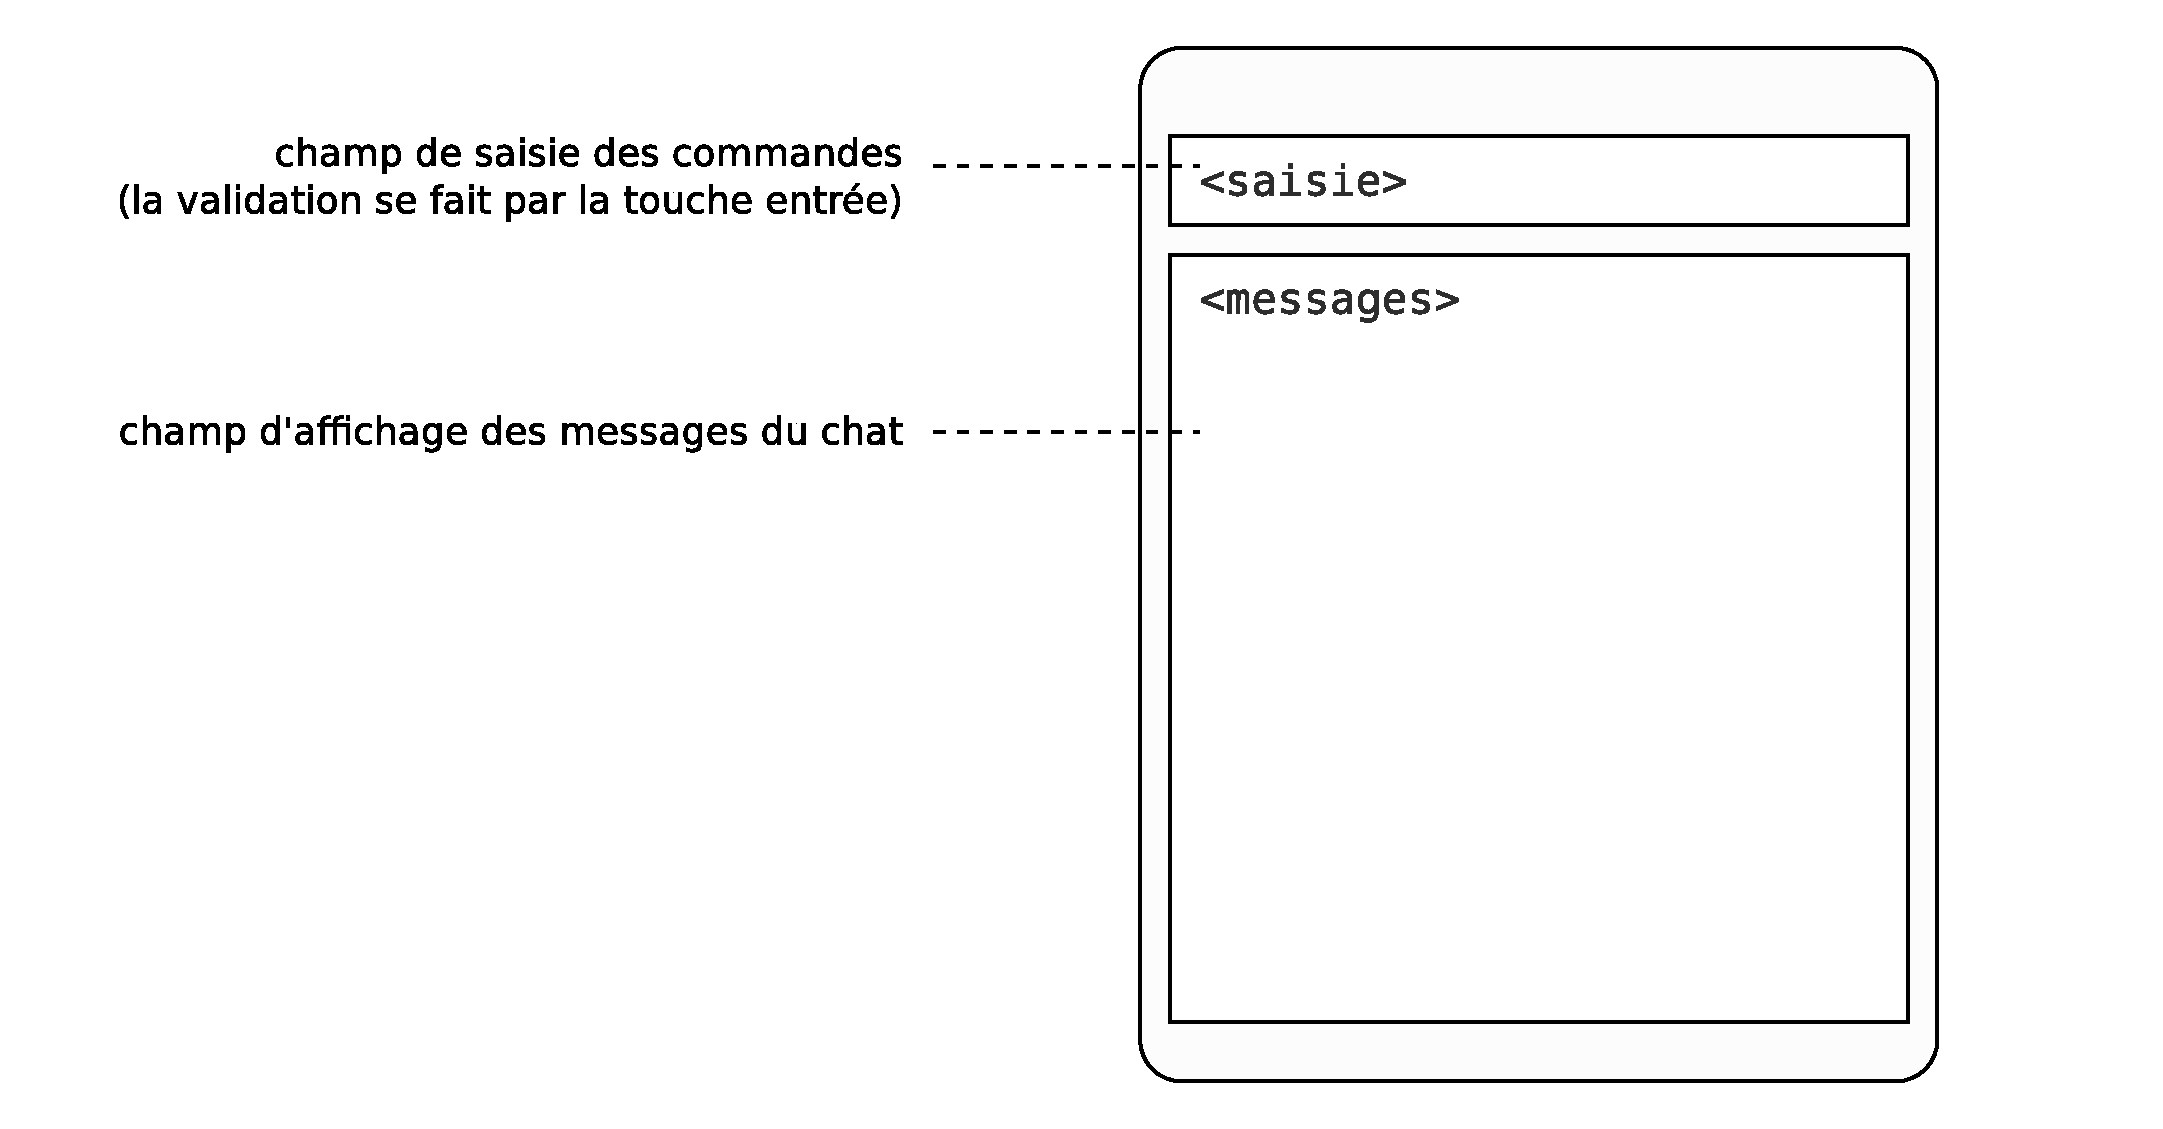
\includegraphics[width=\linewidth]{../img/Chat_IHM.eps}
\caption{IHM du client chat Felix : vue chat.}
\label{sec:ihm:felix:fig}
\end{figure}

\subsection{Protocole de communication client/serveur}
\label{sec:ihm:protocole}

Pour utiliser les différentes fonctionnalités du chat un protocole est à la disposition des utilisateurs.
Ce protocole définit un ensemble de commandes que peut invoquer un utilisateur.

\medskip
Le tableau~\ref{sec:cu:protocole:commandes} énumère les commandes disponibles dans le chat.

\medskip
\begin{table}[h!]
\renewcommand{\arraystretch}{1.3}
\begin{center}
\begin{tabular}{|l|l|}
\hline
   /n \textit{surnom} & Changer de surnom. \\
   /a \textit{nom du canal} & Créer un canal de discussion. \\
   /r \textit{nom du canal} & Supprimer un canal de discussion. \\
   /c \textit{nom du canal} & Changer de canal de discussion. \\
   /l & Afficher la liste des canaux de discussion. \\
   /? & Afficher ses informations personnelles. \\
   /h & Afficher l'aide sur les commandes du chat. \\
\hline
\end{tabular}
\caption{Liste des commandes du chat.}
\label{sec:cu:protocole:commandes}
\end{center}
\end{table}

\subsection{Messages textuels}
\label{sec:ihm:message}

L'utilisation du chat prévoit des messages communiqués aux utilisateurs par le serveur.
Les listings~\ref{sec:ihm:message:arrivee}, page~\pageref{sec:ihm:message:arrivee}, à \ref{sec:ihm:message:suppressionplacepublique}, page~\pageref{sec:ihm:message:suppressionplacepublique}, spécifient ces différents messages.

\bigskip
\begin{lstlisting}[caption={\normalsize{Message d'arrivée d'un utilisateur dans le chat {\footnotesize(à destination de la place publique)}.}},label={sec:ihm:message:arrivee}]
* Un nouvel utilisateur est dans le chat (place publique).
\end{lstlisting}

\medskip
\begin{lstlisting}[caption={\normalsize{Message d'accueil dans le chat.}},label={sec:ihm:message:accueil}]
* Taper /h pour avoir de l'aide sur les commandes du chat.
\end{lstlisting}

\medskip
\begin{lstlisting}[caption={\normalsize{Message d'aide sur les commandes du chat.}},label={sec:ihm:message:aide}]
* Commandes disponibles : 
   /n : changer de surnom ;
   /c : changer de canal ;
   /l : afficher les canaux ;
   /a : créer un canal ;
   /r : supprimer un canal ;
   /? : afficher ses informations ;
   /h : afficher l'aide.
\end{lstlisting}

\medskip
\begin{lstlisting}[caption={\normalsize{Exemple de message transmis dans le chat.}},label={sec:ihm:message:message}]
utilisateur_x > Hello World !

Remarque : Un message est préfixé par le surnom de l'émetteur suivi de '>'.
\end{lstlisting}

\medskip
\begin{lstlisting}[caption={\normalsize{Exemple de message de changement de surnom d'un utilisateur.}},label={sec:ihm:message:surnom}]
* utilisateur_x devient utilisateur_y.
\end{lstlisting}

\medskip
\begin{lstlisting}[caption={\normalsize{Exemple de message sur des informations personnelles.}},label={sec:ihm:message:infoperso}]
* Informations personnelles : 
   Surnom : utilisateur_x
   Canal  : place publique
\end{lstlisting}

\medskip
\begin{lstlisting}[caption={\normalsize{Exemple de message sur des informations sur les canaux.}},label={sec:ihm:message:infocanaux}]
* Canaux disponibles : 
   - canal_x (3)
   - place publique (2)

Remarque : Le nombre d'utilisateurs dans un canal est donné entre parenthèses.
\end{lstlisting}

\medskip
\begin{lstlisting}[caption={\normalsize{Exemple de message de création de canal.}},label={sec:ihm:message:canalcreation}]
* Le canal canal_x a été créé.
\end{lstlisting}

\medskip
\begin{lstlisting}[caption={\normalsize{Exemple de message de création impossible de canal {\footnotesize(le canal existe déjà)}.}},label={sec:ihm:message:}]
* Le canal canal_x existe déjà.
\end{lstlisting}

\medskip
\begin{lstlisting}[caption={\normalsize{Exemple de message de départ d'un canal.}},label={sec:ihm:message:canaldepart}]
* utilisateur_x quitte le canal place publique.
\end{lstlisting}

\medskip
\begin{lstlisting}[caption={\normalsize{Exemple de message d'arrivée dans un canal.}},label={sec:ihm:message:canalarrivee}]
* utilisateur_x rejoint le canal canal_x.
\end{lstlisting}

\medskip
\begin{lstlisting}[caption={\normalsize{Message de non existence d'un canal demandé {\footnotesize(pour changement de canal)}}},label={sec:ihm:message:canalchangementimpossible}]
* Le canal demandé n'existe pas.
\end{lstlisting}

\medskip
\begin{lstlisting}[caption={\normalsize{Exemple de message de suppression d'un canal.}},label={sec:ihm:message:canalsuppression}]
* Le canal canal_x a été supprimé.
\end{lstlisting}

\medskip
\begin{lstlisting}[caption={\normalsize{Exemple de message de suppression impossible d'un canal {\footnotesize(le canal n'existe pas).}}},label={sec:ihm:message:suppressionexistence}]
* Le canal canal_y n'existe pas.
\end{lstlisting}

\medskip
\begin{lstlisting}[caption={\normalsize{Exemple de message de suppression impossible d'un canal {\footnotesize(le canal n'est pas vide).}}},label={sec:ihm:message:canalsuppressionnonvide}]
* Le canal canal_x n'est pas vide.
\end{lstlisting}

\medskip
\begin{lstlisting}[caption={\normalsize{Message de suppression impossible du canal \og place publique \fg.}},label={sec:ihm:message:suppressionplacepublique}]
* Impossible de supprimer le canal par défaut du chat (place publique).
\end{lstlisting}

\medskip
\begin{lstlisting}[caption={\normalsize{Exemple de message de départ d'un utilisateur du chat.}},label={sec:ihm:message:departchat}]
* utilisateur_x quitte le chat.
\end{lstlisting}


\newpage

%--------------------------------------
% Spécifications du chat Felix - Camix
%
% CU
%--------------------------------------

\section{Tests}
\label{sec:t}

\medskip
Dans le cadre du projet, nous avons été amenés à réaliser des tests unitaires et des tests d'intégration.
Ces tests doivent prendre en compte les demandes du client.
Ainsi que toute mise à jour apportée par ce dernier.

\subsection{Specifications demandée par le client}
\label{sec:t:specclient}

Vous pourrez retrouver les spécifications demandées par le client dans la section \ref{sec:cu}.
En revanche dans le cadre du projet, nous avons rédigé des spécifications liées à l'entrée dans le chat en fonction de la mise à jour du client.


\subsection{Entrer dans le chat - MIS A JOUR}
\label{sec:t:entrerchat}

\noindent
Cas d'utilisation : Entrer dans le chat.\\
Résumé : Un utilisateur entre dans le chat en lançant le logiciel client du chat.\\
Acteur principal : Utilisateur.\\
Acteurs secondaires : Les autres utilisateurs du chat.\\
Pré-conditions : Un logiciel serveur (Camix) est lancé et accessible par le réseau TCP/IP.

\medskip
\textbf{Spécifications fonctionnelles avec variantes} :
\begin{enumerate}
\item L'utilisateur lance l'exécution du composant Felix.
\item Felix affiche la vue de connexion au chat.
\item L'utilisateur demande à se connecter.
\item Felix affiche un message de connexion.
\item Retour sur le point d'origine. (2)
    \item Camix inscrit l'utilisateur dans le canal par défaut. (place publique)
    \item Camix envoie un message d'arrivée à tous les utilisateurs du canal par défaut.
    \item Chaque composant Felix affiche le message d'arrivée.
    \item Camix transmet au composant Felix de l'utilisateur un message d'accueil dans le chat.
    \item Felix ferme la vue de connexion au chat.
    \item Felix affiche la vue du chat.
    \item Felix affiche le message d'accueil dans le chat.
\end{enumerate}

\textbf{Variantes :[Modifications de l'addresse IP du serveur]}
\begin{enumerate}
    \item[3.a.1.] L'utilisateur modifie l'adresse IP du serveur.
    \item[3.a.2.] Retour à l'étape 3. de la spécification fonctionnelle.
\end{enumerate}

\textbf{Variantes :[Modification du port du serveur]}
\begin{enumerate}
    \item[3.b.1.] L'utilisateur modifie le port du serveur.
    \item[3.b.2.] Retour à l'étape 3. de la spécification fonctionnelle.
\end{enumerate}

\textbf{Variantes :[Connexion impossible]}
\begin{enumerate}
    \item[6.a.1.] Felix affiche un message de connexion impossible.
    \item[6.a.2.] Retour à l'étape 3. de la spécification fonctionnelle.
\end{enumerate}




\newpage

\end{document}

%--- END 


